\documentclass[10pt,a4paper]{article}
\renewcommand{\baselinestretch}{1.0}
\usepackage{cite}
\usepackage[dvips]{graphicx}
\usepackage{psfrag}
\usepackage{color}
\usepackage[cmex10]{amsmath}
\usepackage{amsfonts}
\usepackage[font=footnotesize, captionskip=10pt]{subfig}
\usepackage{tikz}
\usepackage{flushend}
\usepackage{times}
\usepackage[margin=1.5cm]{geometry}
\usepackage[slovak]{babel}
\usepackage[utf8]{inputenc}
\usepackage[T1]{fontenc}

\usepackage{multirow}
\usepackage{colortbl}

\pagestyle{empty}

\hyphenation{net-works}
\newtheorem{remark}{Remark}

\begin{document}

\title{Deep Q networks}
\author{Michal Chovanec, michal.nand@gmail.com}
\date{}
\maketitle
\thispagestyle{empty}

\section{Q-learning}


\begin{figure}[!htb]
  \centering
  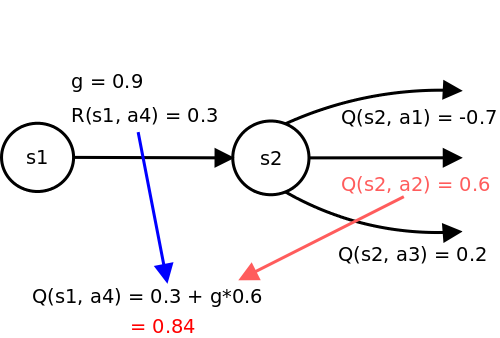
\includegraphics[scale=0.3]{../../diagrams/q_learning_detail.png}
  \caption{Q learning}
  \label{img:q_learning}
\end{figure}

\begin{align}
Q(s, a) = R + \gamma \max \limits_{\alpha'} Q(s', \alpha')
\label{eq:q_learning}
\end{align}

where \\
$s$ is state \\
$a$ is action \\
$s'$ is next state \\
$a'$ is best action in next state \\
$R$ is reward function \\
$\gamma \in \langle 0, 1 \rangle$ is discount factor \\


\section{Deep Q network - DQN}

Approximate $Q(s, a)$ using neural network as $\hat{Q}(s, a; w)$, where $w$ are learnable network
parameters

resulted $Q$ value using \ref{eq:q_learning}
\begin{align}
  \hat{Q}(s, a; w) = R + \gamma \max \limits_{\alpha'} \hat{Q}(s', \alpha'; w)
\end{align}

error to minimize
\begin{align}
  E = \underset{\bf \color{green} target\ value}{R + \gamma \max \limits_{\alpha'} \hat{Q}(s', \alpha'; w)} - \underset{\bf \color{red} predicted\ value}{\hat{Q}(s, a; w) }
\end{align}

weights gradient
\begin{align}
  \Delta w = \eta E \nabla _w \hat{Q}(s, \alpha, w)
\end{align}

There is changing target value, $\hat{Q}(s, a; w)$ depends on $w$ which is also changing during training, and leads to unstable learning.

{\bf Solution - fix $w$}, using temporary network with $w'$ weights. This leads to deep Q learning equation

\begin{align}
  \hat{Q}(s, a; w) = R + \gamma \max \limits_{\alpha'} \hat{Q}(s', \alpha'; w')
  \label{eq:dqn}
\end{align}

and every $K$ steps update $w' \leftarrow w$, usually after training epoch.
For agent decission making, the network $w'$ is used.
Finaly, network error can be computed as
\begin{align}
  E = R + \gamma \max \limits_{\alpha'} \hat{Q}(s', \alpha'; w') - \hat{Q}(s, a; w)
  \label{eq:dqn_error}
\end{align}

Principle of DQN can be demostrated on image \ref{img:dqn} (Q-learning $\gamma$ and $max$ operator are removed for
simplicity).

\begin{figure}[!htb]
  \centering
  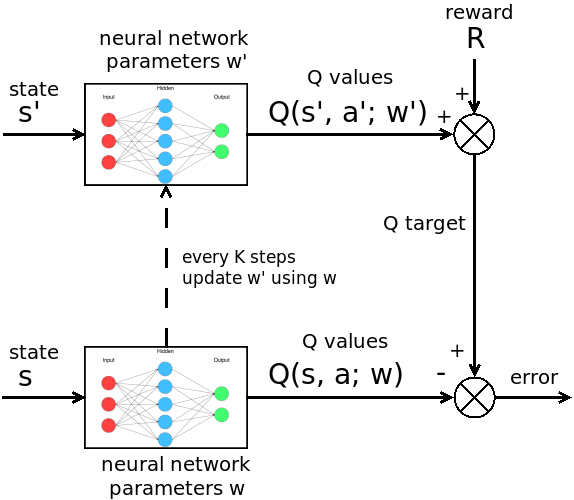
\includegraphics[scale=0.3]{../../diagrams/dqn.png}
  \caption{basic DQN principle}
  \label{img:dqn}
\end{figure}

\section{Dueling deep Q network - DDQN}

\begin{align}
  \hat{Q}(s, a, w) = \underset{\bf \color{green} value\ for\ being\ in\ state\ s}{\hat{V}(s, w)} + \underset{\bf \color{red} advantage\ of\ taking\ action\ a\ at\ state\ s}{\hat{A}(s, a, w)}
\end{align}


\begin{figure}[!htb]
  \centering
  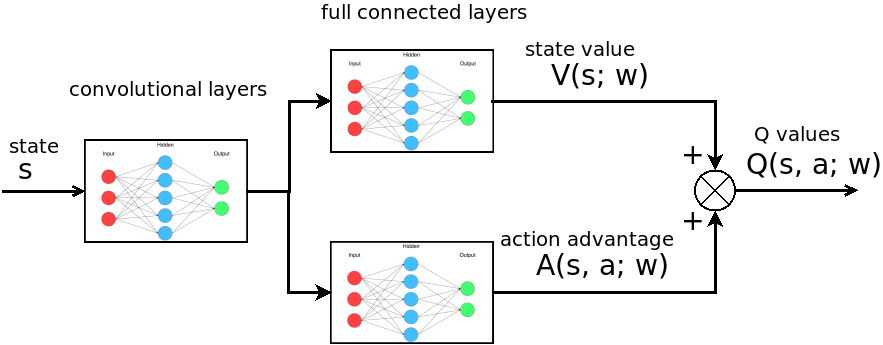
\includegraphics[scale=0.3]{../../diagrams/dueling_dqn_0.png}
  \caption{dueling DQN principle}
  \label{img:ddqn_principle}
\end{figure} 


to avoid identifiability we substract average value of A truth all actions

\begin{align}
  \hat{Q}(s, a, w) = \hat{V}(s, w) + \hat{A}(s, a, w) - \frac{1}{N_{\alpha'}} \sum_{\alpha'} \hat{A}(s, \alpha', w)
\end{align}

using equation \ref{eq:dqn} we obtain dueling deep Q network equation

\begin{align}
  \hat{Q}(s, a; w) = R + \gamma \left( \hat{V}(s', w') + \max \limits_{\alpha'} \hat{A}(s', \alpha', w') - \frac{1}{N_{\alpha'}} \sum_{\alpha'} \hat{A}(s', \alpha', w') \right)
  \label{eq:ddqn}
\end{align}

and finally the weights learning rule

\begin{align}
  \Delta w = \eta \left( R + \gamma \left( \hat{V}(s', w') + \max \limits_{\alpha'} \hat{A}(s', \alpha', w') - \frac{1}{N_{\alpha'}} \sum_{\alpha'} \hat{A}(s', \alpha', w') \right) - \hat{Q}(s, a; w)\right) \nabla_w \hat{Q}(s, a; w)
  \label{eq:ddqn_w_update}
\end{align}


\begin{figure}[!htb]
  \centering
  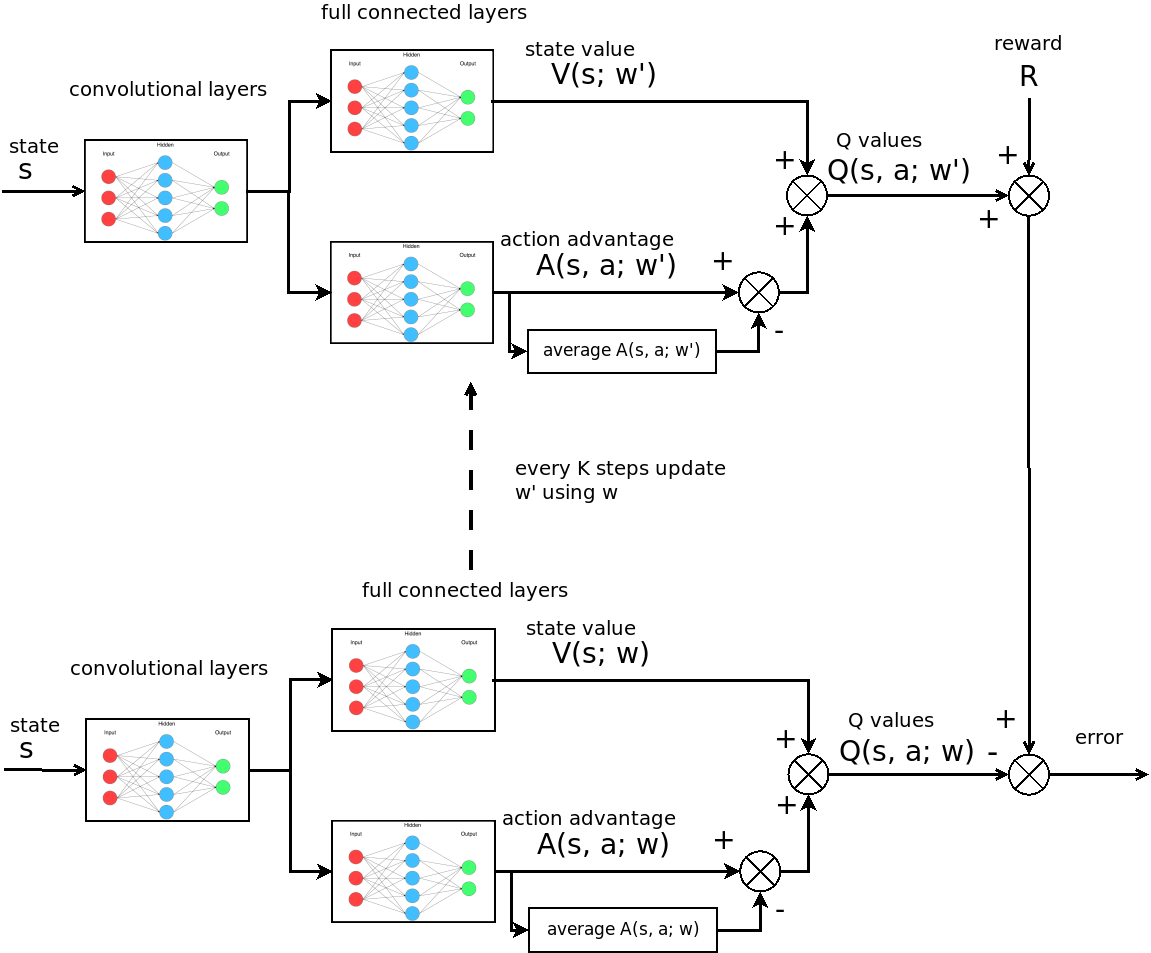
\includegraphics[scale=0.3]{../../diagrams/dueling_dqn_1.png}
  \caption{dueling DQN principle, full}
  \label{img:ddqn_full}
\end{figure}


\newpage
\section{Experiments}

\begin{figure}[!htb]
  \centering
  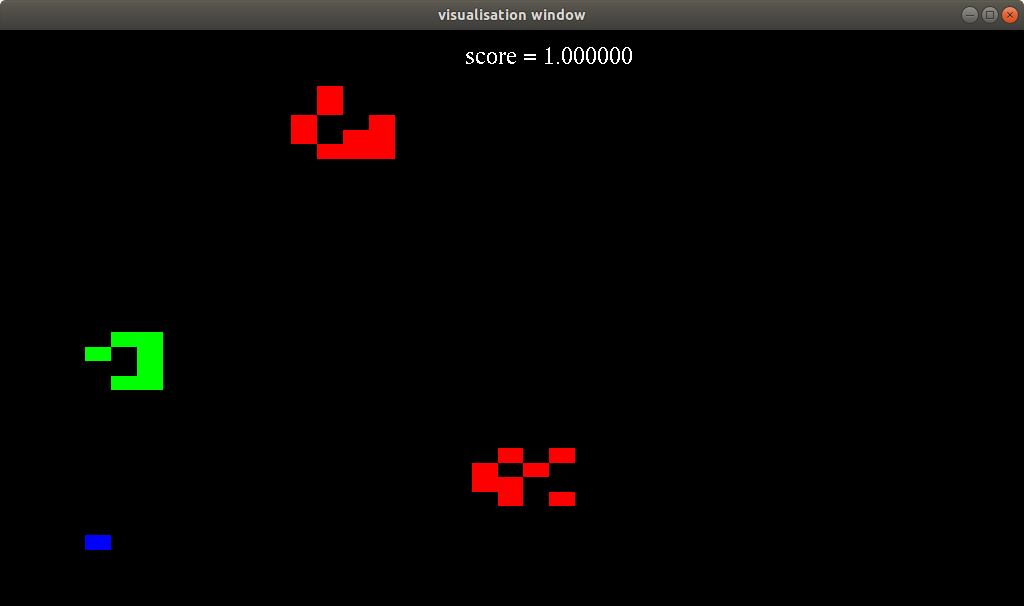
\includegraphics[scale=0.25]{../../diagrams/arcade_obstacles.png}
  \caption{example of testing game}
  \label{img:dqn_test_game}
\end{figure}

Network hyperparameters
\begin{itemize}
  \item init weights  : XAVIER
  \item learning rate : 0.0005
  \item L1 regularization : 0.0000001
  \item L2 regularization : 0.0000001
  \item dropout           : 0.2,
  \item minibatch size    : 32
\end{itemize}

RL hyperparameters
\begin{itemize}
  \item experience buffer size  : 1024
  \item gamma : 0.9
  \item epsilon training : 0.2
  \item epsilon testing : 0.05
\end{itemize}

\begin{table}[]
\centering
\begin{tabular}{|l|c|c|}
\hline
\textbf{layer type}                       & \textbf{input dimensions} & \textbf{kernel dimensions} \\ \hline
\cellcolor[HTML]{CBCEFB}dense convolution & 16x32x3                   & 3x3x8                      \\ \hline
\cellcolor[HTML]{CBCEFB}dense convolution & 16x32x11                  & 3x3x8                      \\ \hline
\cellcolor[HTML]{CBCEFB}dense convolution & 16x32x19                  & 3x3x8                      \\ \hline
\cellcolor[HTML]{CBCEFB}dense convolution & 16x32x27                  & 3x3x8                      \\ \hline
\cellcolor[HTML]{67FD9A}convolution       & 16x32x35                  & 3x3x32                     \\ \hline
\cellcolor[HTML]{FD6864}full connected    & 16x32x32                  & actions\_count             \\ \hline
\end{tabular}
\caption{testing network architecture}
\label{tab:dqn_test_network_architecture}
\end{table}

\begin{figure}[!htb]
  \centering
  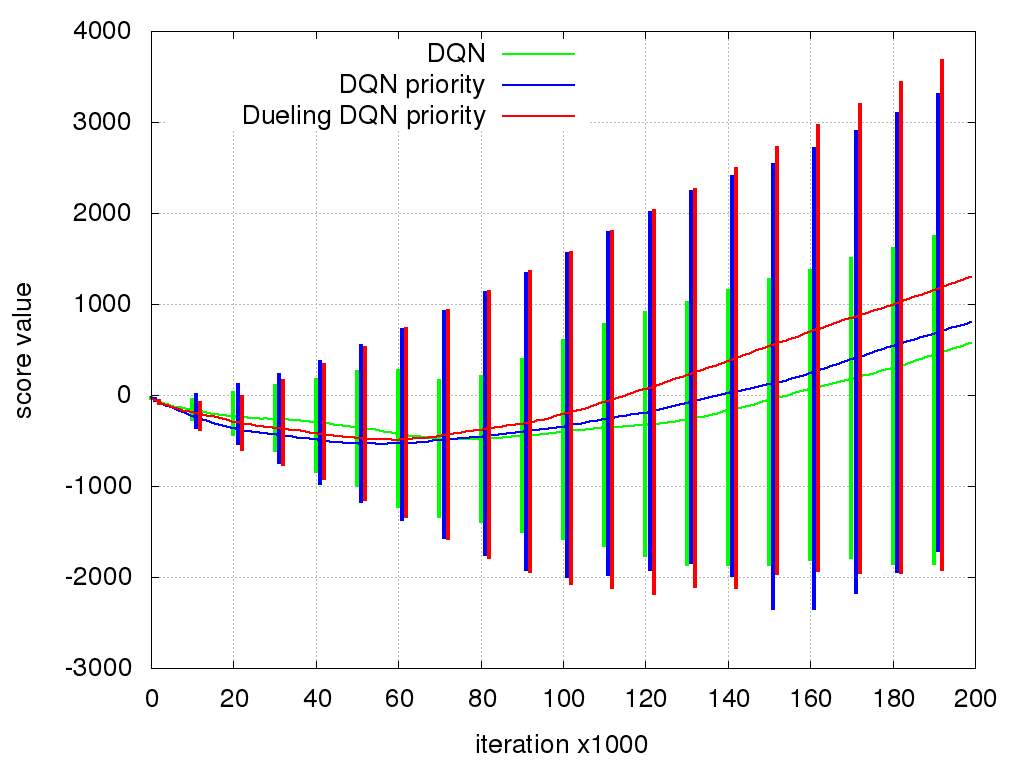
\includegraphics[scale=0.4]{../../rl_results/dqn_test/rl_progress_training.png}
  \caption{training score progress}
  \label{img:dqn_test_training_progress}
\end{figure}


\begin{figure}[!htb]
  \centering
  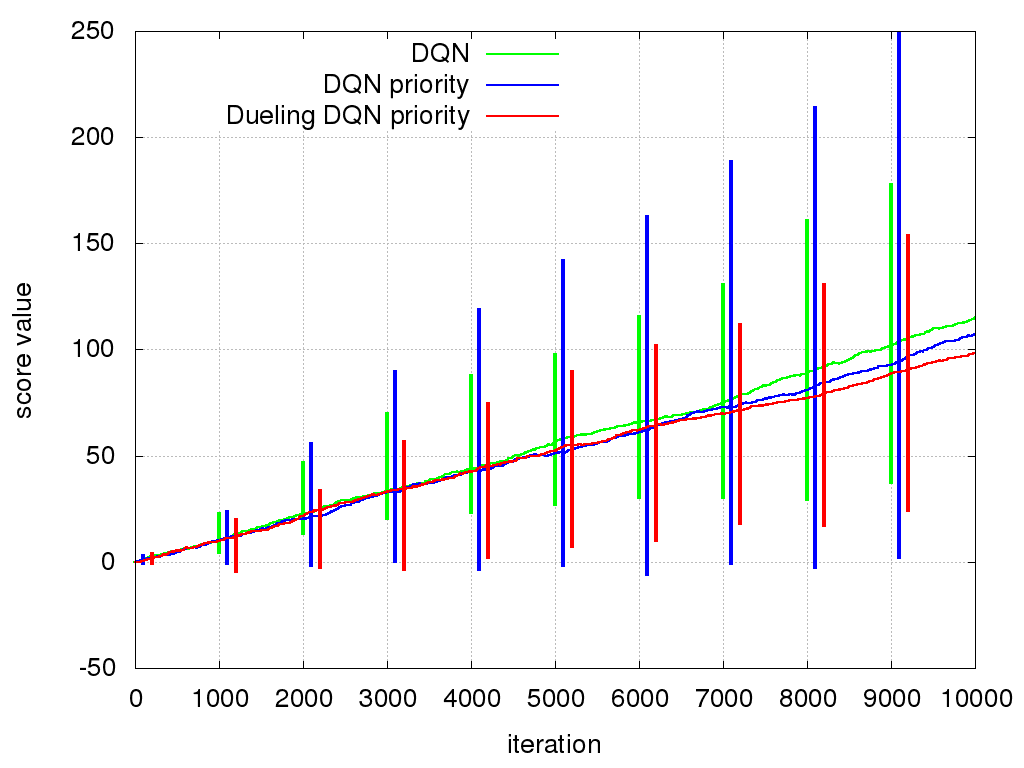
\includegraphics[scale=0.4]{../../rl_results/dqn_test/rl_progress_testing.png}
  \caption{testing score progress}
  \label{img:dqn_test_testing_progress}
\end{figure}



\end{document}
